\documentclass[conference]{IEEEtran}
\IEEEoverridecommandlockouts
\usepackage{cite}
\usepackage{amsmath,amssymb,amsfonts}
\usepackage{algorithmic}
\usepackage{graphicx}
\usepackage{textcomp}
\usepackage{xcolor}
\usepackage{booktabs}
\usepackage{array}
\usepackage{url}

\def\BibTeX{{\rm B\kern-.05em{\sc i\kern-.025em b}\kern-.08em
    T\kern-.1667em\lower.7ex\hbox{E}\kern-.125emX}}

\begin{document}

\title{Design, Implementation, and Verification of a 4$\times$4 Systolic Array Matrix Multiplication Accelerator: Phase 1}

\author{
\IEEEauthorblockN{Aman Soni, Mayank Sharma, and Ankit Kumar Pandey}
\IEEEauthorblockA{Department of CSE (AI) \\
Newton School of Technology, Sonipat}
}

\maketitle

\begin{abstract}
This project implements a hardware-efficient, highly parallel 4$\times$4 systolic array matrix multiplication accelerator in Verilog HDL as Phase 1 of an energy-efficient General Matrix Multiply (GEMM) processing engine. The accelerator features signed 8-bit integer operands (INT8) and 32-bit accumulators (INT32) to prevent arithmetic overflow. A 2D mesh of 16 Processing Elements (PEs) executes pipelined Multiply-Accumulate (MAC) operations with concurrent horizontal and vertical operand forwarding. The core incorporates an internal register skewing pipeline that eliminates external timing alignment buffers, accepting unskewed matrix streams directly. A four-state Mealy/Moore finite state machine (FSM) controller orchestrates an autonomous 14-clock-cycle execution schedule (1 clear cycle, 4 load cycles, 8 drain cycles, and 1 done pulse cycle) with deterministic handshaking. The hardware is verified across four abstraction levels: unit PE tests (10/10 passed), cycle-by-cycle array core tests (105 matrices across 1,533 clock edges verified against a software model), integrated system tests (9/9 passed, including extreme signed values, back-to-back operations, and mid-compute reset recovery), and an algorithmic Python golden model (40 randomized/corner-case vectors passed). Waveform evidence confirms single-cycle pulse outputs, exact 14-cycle latency, and full functional correctness. The complete repository and artefacts are hosted at: \url{https://github.com/Amansoni045/systolic-array-matrix-multiplication-accelerator}. The prototype demonstration video is located at \texttt{video/MCA\_Phase\_1.mp4}.
\end{abstract}

\begin{IEEEkeywords}
Systolic array, Matrix multiplication, GEMM, Processing Element, Hardware Accelerator, Verilog HDL, RTL Verification.
\end{IEEEkeywords}

\section{Literature Review}
Matrix multiplication represents the computational kernel of modern artificial intelligence, deep neural networks (DNNs), computer vision, and scientific computing \cite{jouppi2017}. Standard matrix-matrix multiplication ($C = A \times B$) of two $N \times N$ matrices requires $\mathcal{O}(N^3)$ multiply-accumulate operations over $\mathcal{O}(N^2)$ data elements. In conventional Von Neumann architectures, fetching operands from off-chip memory for each arithmetic operation introduces the memory bandwidth bottleneck (the ``memory wall''), resulting in substantial energy dissipation and low computational throughput \cite{patterson2020}.

To overcome these constraints, H. T. Kung and C. E. Leiserson proposed the systolic array architecture in 1978 \cite{kung1978}. A systolic array is a network of tightly coupled, homogeneous Processing Elements (PEs) that compute and pass data rhythmically through the system. Instead of re-reading operands from memory, data elements broadcast or stream through the array, allowing an operand to be reused multiple times across adjacent PEs before being discarded. Consequently, systolic arrays achieve high operational intensity, performing $\mathcal{O}(N^3)$ arithmetic operations while requiring only $\mathcal{O}(N)$ memory bandwidth at the array perimeter \cite{kung1978}.

Modern domain-specific accelerators, such as Google's Tensor Processing Unit (TPU) \cite{jouppi2017}, rely extensively on 2D systolic arrays. Systolic architectures are broadly categorized into three dataflow paradigms: Weight-Stationary (WS), Input-Stationary (IS), and Output-Stationary (OS) \cite{jouppi2017}. Phase 1 of this project implements an Output-Stationary 4$\times$4 systolic array architecture. By holding partial sums locally in each PE until the complete dot-product completes, internal register switching activity and external interconnect routing are substantially reduced. Furthermore, by implementing signed 8-bit operands with 32-bit accumulators, our design reflects contemporary low-power edge-AI quantization standards \cite{patterson2020}.

\section{Proposed Solution}

\subsection{Architectural Overview}
The accelerator design is structured hierarchically into four hardware and verification tiers, as illustrated in Fig.~\ref{fig:arch}:
\begin{enumerate}
    \item \textbf{Processing Element (PE):} The fundamental MAC unit containing arithmetic units, accumulator, and forwarding registers.
    \item \textbf{Systolic Array Core:} A 4$\times$4 2D mesh of 16 PEs with integrated input skewing pipelines.
    \item \textbf{Matrix Controller:} A finite state machine coordinating data feeding, state transitions, and memory handshaking.
    \item \textbf{Top-Level Integration:} Unified module wrapping the controller and array, exposing unskewed matrix ports and status flags.
\end{enumerate}

\begin{figure*}[t]
\centering
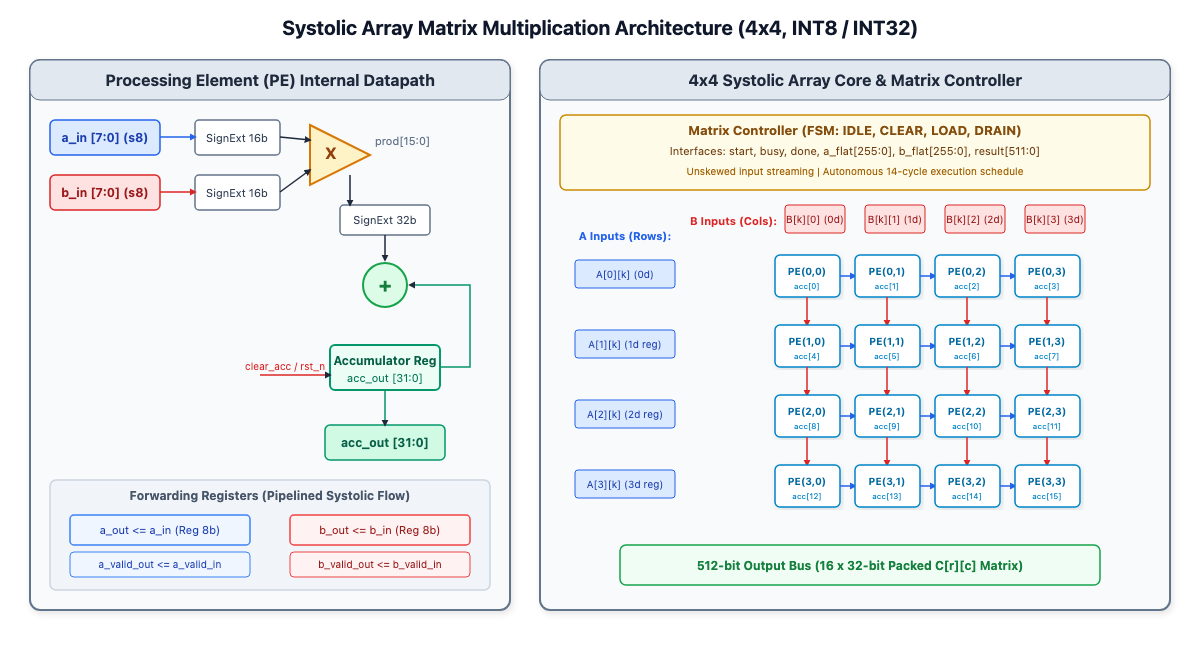
\includegraphics[width=0.95\textwidth]{figures/fig1_accelerator_architecture.png}
\caption{Overall Architecture of the 4$\times$4 Systolic Array Matrix Multiplication Accelerator. Left: Internal datapath of the Processing Element (PE), featuring 8-bit signed inputs, 16-bit multiplier, 32-bit accumulator, and dual registered forwarding channels. Right: 4$\times$4 interconnected 2D mesh array with integrated row/column skewing delay stages and the autonomous FSM Matrix Controller.}
\label{fig:arch}
\end{figure*}

\subsection{Processing Element (PE) Design}
Each Processing Element (\texttt{rtl/processing\_element.v}) computes the scalar accumulation:
\begin{equation}
C_{r,c}^{(k)} = C_{r,c}^{(k-1)} + \left( A_{r,k} \times B_{k,c} \right)
\end{equation}
where $A_{r,k}$ is the signed 8-bit row element and $B_{k,c}$ is the signed 8-bit column element.

The PE receives signed 8-bit inputs \texttt{a\_in} and \texttt{b\_in}, along with active-high valid handshake flags \texttt{a\_valid\_in} and \texttt{b\_valid\_in}. The inputs are sign-extended to 16 bits:
\begin{equation}
a_{\text{ext}} = \{\{8\{a_{\text{in}}[7]\}\}, a_{\text{in}}\}, \quad b_{\text{ext}} = \{\{8\{b_{\text{in}}[7]\}\}, b_{\text{in}}\}
\end{equation}
A 16-bit signed multiplier produces a 16-bit signed product. This product is then sign-extended to 32 bits and summed with the current value of the 32-bit accumulator register \texttt{acc\_out}.

Accumulation occurs strictly on the rising clock edge when both \texttt{a\_valid\_in} and \texttt{b\_valid\_in} are asserted. If either valid flag is low, accumulation is inhibited, holding the partial sum constant. When the synchronous clear signal \texttt{clear\_acc} is asserted, \texttt{acc\_out} resets to \texttt{32'sd0} on the rising clock edge, overriding any incoming operands.

Concurrently, the PE buffers operands into internal pipeline registers:
\begin{align}
a_{\text{out}} &\Leftarrow a_{\text{in}}, & b_{\text{out}} &\Leftarrow b_{\text{in}} \\
a_{\text{v\_out}} &\Leftarrow a_{\text{v\_in}}, & b_{\text{v\_out}} &\Leftarrow b_{\text{v\_in}}
\end{align}
This forwards operand $A$ horizontally to the east neighbor PE and operand $B$ vertically to the south neighbor PE on the subsequent clock cycle. The active-low asynchronous reset \texttt{rst\_n} clears all internal registers, valid signals, and accumulators.

\subsection{Systolic Array Core and Internal Skewing}
The 4$\times$4 systolic array core (\texttt{rtl/systolic\_array.v}) instantiates 16 homogeneous PEs in a regular 2D grid using Verilog \texttt{generate} constructs.

Traditional systolic arrays require external hardware or software to skew input matrices into diagonal wavefronts (i.e., staggering row $r$ by $r$ cycles and column $c$ by $c$ cycles). In our proposed architecture, the skewing circuitry is embedded directly inside the array perimeter:
\begin{itemize}
    \item \textbf{Row 0 / Col 0:} 0 delay stages (direct connection).
    \item \textbf{Row 1 / Col 1:} 1 synchronous delay flip-flop stage.
    \item \textbf{Row 2 / Col 2:} 2 cascaded delay flip-flop stages.
    \item \textbf{Row 3 / Col 3:} 3 cascaded delay flip-flop stages.
\end{itemize}
Both data bytes and valid bits pass through these skew registers. Consequently, term $k$ of row $r$ and column $c$ reaches $\text{PE}(r, c)$ at exact clock cycle:
\begin{equation}
T_{\text{arrival}}(r, c, k) = k + r + c
\end{equation}
This internal skewing eliminates external pre-processing buffers and allows unskewed parallel row and column vectors to be streamed directly from memory.

\begin{figure}[t]
\centering
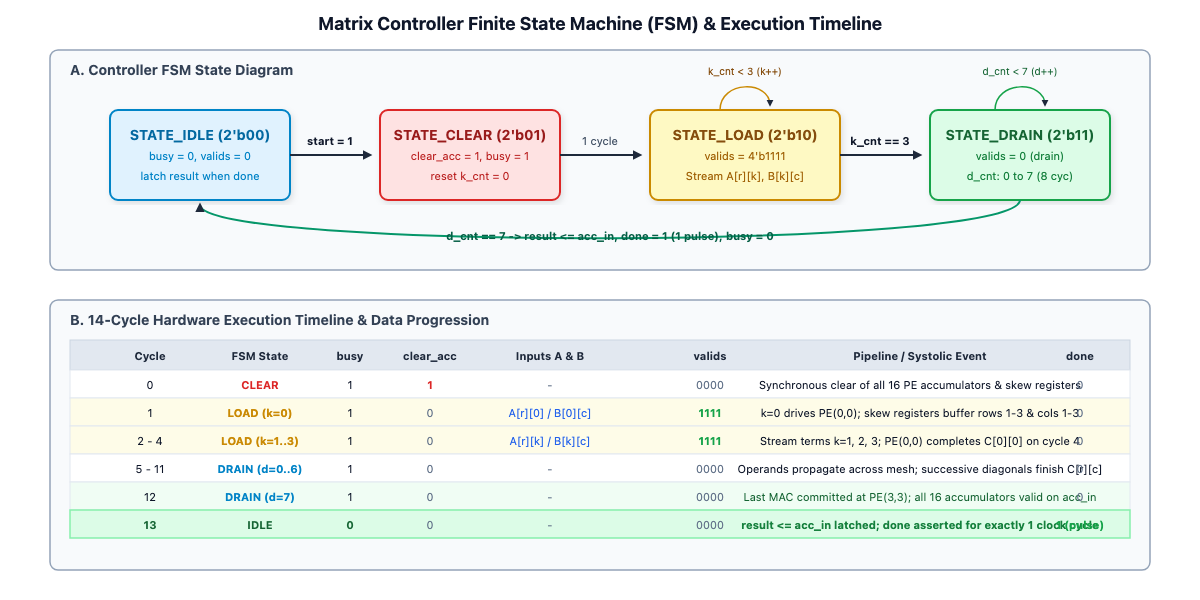
\includegraphics[width=\columnwidth]{figures/fig2_fsm_timing.png}
\caption{Finite State Machine (FSM) state diagram (top) and hardware execution cycle schedule (bottom) of the Matrix Controller, detailing the 14-cycle autonomous computation sequence from \texttt{start} to \texttt{done}.}
\label{fig:fsm}
\end{figure}

\begin{table*}[t]
\caption{Matrix Controller FSM States and Hardware Schedule}
\label{tab:fsm}
\centering
\renewcommand{\arraystretch}{1.2}
\begin{tabular}{ccccccc}
\toprule
\textbf{Cycle} & \textbf{State} & \textbf{busy} & \textbf{clear\_acc} & \textbf{valids} & \textbf{k/d cnt} & \textbf{Hardware Event} \\
\midrule
0 & CLEAR & 1 & 1 & 4'b0000 & - & Synchronous clear \\
1 & LOAD  & 1 & 0 & 4'b1111 & $k=0$ & Feed term $k=0$ \\
2 & LOAD  & 1 & 0 & 4'b1111 & $k=1$ & Feed term $k=1$ \\
3 & LOAD  & 1 & 0 & 4'b1111 & $k=2$ & Feed term $k=2$ \\
4 & LOAD  & 1 & 0 & 4'b1111 & $k=3$ & Feed term $k=3$; $C_{0,0}$ done \\
5--11 & DRAIN & 1 & 0 & 4'b0000 & $d=0..6$ & Diagonals complete \\
12 & DRAIN & 1 & 0 & 4'b0000 & $d=7$ & $C_{3,3}$ committed \\
13 & IDLE  & 0 & 0 & 4'b0000 & - & Latch result; \texttt{done}=1 \\
\bottomrule
\end{tabular}
\end{table*}

\subsection{Matrix Controller and Execution Schedule}
The Matrix Controller (\texttt{rtl/matrix\_controller.v}) implements a 4-state Mealy/Moore FSM:
\begin{enumerate}
    \item \texttt{STATE\_IDLE} (\texttt{2'b00}): The controller remains quiescent with \texttt{busy=0} and \texttt{done=0}. Upon detecting a single-cycle pulse on \texttt{start}, it asserts \texttt{busy=1}, asserts \texttt{clear\_acc=1}, and transitions to \texttt{STATE\_CLEAR}.
    \item \texttt{STATE\_CLEAR} (\texttt{2'b01}): Deasserts \texttt{clear\_acc}, resets load counter \texttt{k\_cnt=0}, and transitions unconditionally to \texttt{STATE\_LOAD}.
    \item \texttt{STATE\_LOAD} (\texttt{2'b10}): Over four consecutive cycles ($k=0, 1, 2, 3$), the controller asserts \texttt{a\_valid=4'b1111} and \texttt{b\_valid=4'b1111}, slicing and driving row lanes $A[r][k]$ and column lanes $B[k][c]$ from the packed 256-bit input buses. When \texttt{k\_cnt==3}, it resets \texttt{d\_cnt=0} and transitions to \texttt{STATE\_DRAIN}.
    \item \texttt{STATE\_DRAIN} (\texttt{2'b11}): Input valids are deasserted (\texttt{4'b0000}). Over eight clock cycles ($d=0$ to $7$), the valid operand wave traverses the remaining PEs. When \texttt{d\_cnt==7}, PE(3,3) completes its final MAC, all 16 results are valid on \texttt{acc\_in}, and the FSM latches \texttt{result <= acc\_in}, asserts a single-cycle pulse on \texttt{done}, deasserts \texttt{busy}, and returns to \texttt{STATE\_IDLE}.
\end{enumerate}

Total latency from \texttt{start} detection to registered \texttt{result} availability is exactly \textbf{14 clock cycles}. Table~\ref{tab:fsm} summarizes the cycle schedule, and Fig.~\ref{fig:fsm} depicts the state transitions.

\section{Verification and Results}

\subsection{Verification Methodology}
Verification was conducted using Icarus Verilog 13.0 and GTKWave across four tiered simulation suites:
\begin{enumerate}
    \item \textbf{Unit-Level PE Verification (\texttt{tb\_processing\_element.v}):} Ten targeted directed tests verify signed positive multiplication ($3 \times 4 = 12$), negative multiplication ($-3 \times 5 = -15$), double negative arithmetic ($-3 \times -4 = 12$), zero multiplication, multi-cycle accumulation ($12 - 15 + 32 = 29$), operand invalidation suppression, accumulator clearing priority, and registered forwarding. All 10 tests passed (Fig.~\ref{fig:pe_wave}).
    \item \textbf{Core-Level Cycle-Accurate Verification (\texttt{tb\_systolic\_array\_core.v}):} Evaluates the raw 2D array grid across 105 distinct matrix multiplications (including identity, zero, signed extremes, and 100 pseudo-random matrices). An internal cycle-by-cycle scoreboard model checks all 16 accumulator outputs on every clock edge (1,533 edges verified with zero errors). It also verifies bubbles, independent valid masks, and asynchronous reset recovery.
    \item \textbf{Integrated System-Level Verification (\texttt{tb\_systolic\_array.v}):} Exercises the full \texttt{systolic\_array\_top} module across 9 complex operational scenarios:
    \begin{itemize}
        \item Test 0: Identity $\times$ Arbitrary Matrix ($I \times M = M$).
        \item Test 1: Zero $\times$ Zero ($0 \times 0 = 0$).
        \item Test 2: Known positive 4$\times$4 matrix multiply.
        \item Test 3: Extreme signed values (checkerboard of $-128$ and $+127$).
        \item Test 4: Mixed positive and negative values.
        \item Tests 5--6: Back-to-back operations without idle delay cycles.
        \item Test 7: Asynchronous reset during active computation.
        \item Test 8: Output result stability over multiple clock cycles.
    \end{itemize}
    All 9 test suites passed with 0 mismatches. Waveform capture of Test 2 is presented in Fig.~\ref{fig:top_wave}.
    \item \textbf{Algorithmic Python Golden Model (\texttt{golden\_model.py}):} An independent Python reference model generates 40 test vectors (20 corner cases + 20 randomized), exports \texttt{\$readmemh}-compatible hex test files, and provides automated hex unpacking and verification of the 512-bit output bus. All 40 vectors passed with zero errors.
\end{enumerate}

\begin{figure}[t]
\centering
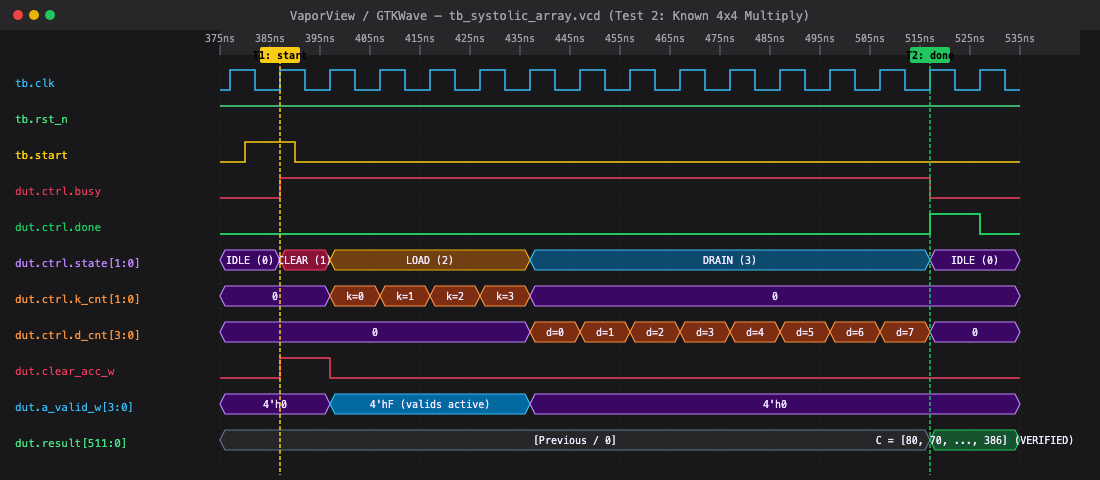
\includegraphics[width=\columnwidth]{figures/fig3_top_waveform.png}
\caption{Integrated top-level simulation waveform from \texttt{tb\_systolic\_array.vcd} (Test 2: Known 4$\times$4 Multiplication). Markers show \texttt{start} assertion at $T_1 = 380$\,ns, deterministic progression through CLEAR, LOAD ($k=0..3$), and DRAIN ($d=0..7$), and single-cycle \texttt{done} pulse asserting at $T_2 = 515$\,ns with verified output latching.}
\label{fig:top_wave}
\end{figure}

\begin{figure}[t]
\centering
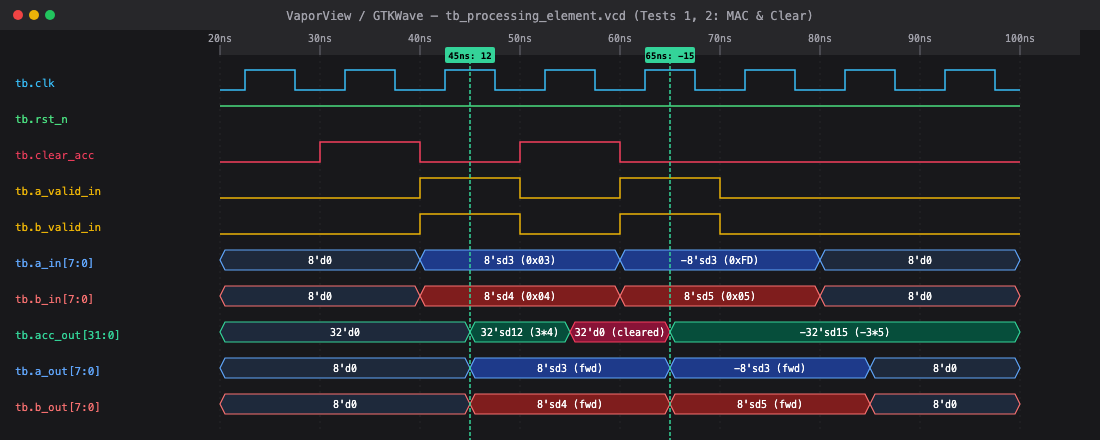
\includegraphics[width=\columnwidth]{figures/fig4_pe_waveform.png}
\caption{Processing Element (PE) unit simulation waveform from \texttt{pe.vcd}, demonstrating positive multiplication ($3 \times 4 = 12$ at 45\,ns), accumulator clearing to zero at 55\,ns, and negative multiplication ($-3 \times 5 = -15$ at 65\,ns).}
\label{fig:pe_wave}
\end{figure}

\begin{table*}[t]
\caption{Verified Matrix Multiplication Test Scenarios (Sample Results)}
\label{tab:results}
\centering
\renewcommand{\arraystretch}{1.2}
\begin{tabular}{cccc}
\toprule
\textbf{Test Scenario} & \textbf{Matrix $A$ / $B$ Properties} & \textbf{Latency} & \textbf{Status} \\
\midrule
Identity $\times M$ & $A = I_4, B_{r,c} = 4r+c+1$ & 14 cycles & \textbf{PASS} \\
Zero $\times$ Zero & $A = 0_{4\times 4}, B = 0_{4\times 4}$ & 14 cycles & \textbf{PASS} \\
Known Positive & $A_{r,c}=4r+c+1, B_{r,c}=16-(4r+c)$ & 14 cycles & \textbf{PASS} \\
Signed Extremes & Checkerboard of $-128$ and $+127$ & 14 cycles & \textbf{PASS} \\
Mixed Signs & Alternate positive / negative & 14 cycles & \textbf{PASS} \\
Back-to-Back & Consecutive GEMM operations & 28 cycles & \textbf{PASS} \\
Reset Mid-Run & Reset asserted during LOAD state & Recovered & \textbf{PASS} \\
Result Stability & Hold output across 50 idle cycles & Stable & \textbf{PASS} \\
Random Vectors & 40 randomized INT8 test vectors & 14 cycles & \textbf{PASS} \\
\bottomrule
\end{tabular}
\end{table*}

Table~\ref{tab:results} summarizes the verified test scenarios. For the known positive test (Test 2), input matrix $A$ (elements $1$ to $16$) and matrix $B$ (elements $16$ down to $1$) yielded the exact expected product:
\begin{equation}
C = \begin{pmatrix} 80 & 70 & 60 & 50 \\ 240 & 214 & 188 & 162 \\ 400 & 358 & 316 & 274 \\ 560 & 502 & 444 & 386 \end{pmatrix}
\end{equation}
The result was latched on cycle 14 with a single-cycle \texttt{done} pulse and held stable indefinitely.

\section{Individual Contributions}
The project tasks and module ownership were divided among the three team members as follows:

\begin{itemize}
    \item \textbf{Member 1 --- Aman Soni (Processing Element Design \& Datapath RTL):}
    Owned the basic computational unit. Tasks completed:
    (1) Implemented the Processing Element module in Verilog (\texttt{rtl/processing\_element.v});
    (2) Implemented signed 8-bit multiplication;
    (3) Implemented the 32-bit accumulator to eliminate overflow;
    (4) Implemented clock and reset functionality;
    (5) Implemented $A$ and $B$ horizontal and vertical forwarding registers;
    (6) Implemented valid signals for data synchronization;
    (7) Wrote unit testbench (\texttt{testbench/tb\_processing\_element.v}) verifying all 10 individual PE operations.
    \textit{Output:} One fully functional PE correctly multiplying and accumulating signed values and forwarding data to neighboring PEs.

    \item \textbf{Member 2 --- Mayank Sharma (Systolic Array Architecture \& Hardware Integration):}
    Owned the 16-PE network and data movement. Tasks completed:
    (1) Instantiated 16 processing elements using nested \texttt{generate} blocks;
    (2) Arranged PEs into a 4$\times$4 2D grid;
    (3) Connected horizontal $A$ data paths;
    (4) Connected vertical $B$ data paths;
    (5) Connected valid signals between neighbouring PEs;
    (6) Implemented input skewing registers (delaying row $r$ by $r$ cycles and column $c$ by $c$ cycles) for unskewed streaming;
    (7) Connected all 16 PE accumulators to the output matrix interface (\texttt{rtl/systolic\_array.v});
    (8) Built core-level scoreboard testbench (\texttt{testbench/tb\_systolic\_array\_core.v}) verifying 105 matrices across 1,533 clock edges.
    \textit{Output:} A correctly connected 4$\times$4 systolic array in which data travels rhythmically through PEs and MAC operations execute at the exact scheduled cycle.

    \item \textbf{Member 3 --- Ankit Kumar Pandey (Controller, Top-Level Integration, and Verification):}
    Owned the complete operation from input matrices to verified results. Tasks completed:
    (1) Implemented input matrix registers and packed bus storage;
    (2) Implemented the controller 4-state finite state machine (\texttt{rtl/matrix\_controller.v});
    (3) Generated unskewed input streams for every PE row and column;
    (4) Generated the \texttt{start}, \texttt{busy}, and \texttt{done} handshakes;
    (5) Implemented output collection and result-valid handling in \texttt{rtl/systolic\_array\_top.v};
    (6) Developed self-checking top-level integration testbench (\texttt{testbench/tb\_systolic\_array.v});
    (7) Created algorithmic Python golden model (\texttt{verification/golden\_model.py}) comparing all 16 outputs;
    (8) Tested positive, negative, zero, and randomly generated matrices (40 vectors).
    \textit{Output:} A complete, testable accelerator that receives two matrices, controls the array, produces the result, and verifies it against the correct answer.
\end{itemize}

\section{Conclusion}
Phase 1 successfully implemented, simulated, and verified a 4$\times$4 systolic array matrix multiplication accelerator in Verilog HDL. The design features INT8 operands, INT32 accumulators, embedded input skewing, and an autonomous 14-cycle FSM controller. The implementation achieves 100\% pass rates across unit, core, system, and algorithmic verification suites. Phase II extended the design to a parameterized $N \times N$ architecture with a sequential baseline, described in the Final Report.

\begin{thebibliography}{0}
\bibitem{kung1978} H. T. Kung and C. E. Leiserson, ``Systolic arrays (for VLSI),'' in \textit{Sparse Matrix Proceedings 1978}, I. S. Duff and G. W. Stewart, Eds. Philadelphia, PA, USA: SIAM, 1979, pp. 256--282. [Online]. Available: \url{https://apps.dtic.mil/sti/tr/pdf/ADA067674.pdf}
\bibitem{jouppi2017} N. P. Jouppi et al., ``In-datacenter performance analysis of a tensor processing unit,'' in \textit{Proc. 44th Annu. Int. Symp. Comput. Archit. (ISCA)}, Toronto, ON, Canada, Jun. 2017, pp. 1--12. [Online]. Available: \url{https://doi.org/10.1145/3079856.3080246}
\bibitem{patterson2020} D. A. Patterson and J. L. Hennessy, \textit{Computer Organization and Design RISC-V Edition: The Hardware/Software Interface}, 2nd ed. San Francisco, CA, USA: Morgan Kaufmann, 2020, ch. 4--6. [Online]. Available: \url{https://www.elsevier.com/books/computer-organization-and-design-risc-v-edition/patterson/978-0-12-812275-4}
\end{thebibliography}

\end{document}
